\documentclass[10pt,a4paper]{article}
\usepackage[margin=2.1cm]{geometry}
\usepackage{amsmath,amssymb,bm}
\usepackage{graphicx,booktabs,xcolor,enumitem,hyperref}
\hypersetup{colorlinks,linkcolor=blue!50!black,urlcolor=blue!50!black}
\newcommand{\ka}{\kappa_1}
\newcommand{\kc}{\kappa_2}
\newcommand{\note}[1]{\par\smallskip\noindent\colorbox{gray!12}{\parbox{\dimexpr\linewidth-2\fboxsep}{\small #1}}\par\smallskip}
\newcommand{\evd}[1]{\textsf{\small[#1]}}
\newcommand{\simple}[1]{\par\noindent\textbf{In simple words:} #1\par\smallskip}
\title{TOP-Q --- Day 2 worked notes\\[2pt]\large Chiral symmetry, winding number, edge states and localisation length}
\author{PH 5110 term paper --- Kotapati Kishore (EE26E016)}
\date{23 October 2026}
\begin{document}\sloppy\maketitle

\note{Same rules as Day 1: re-derive Sections 1--6 on paper without looking. Every result is labelled
\evd{Derived}, \evd{Verified-by-test}, \evd{Simulated}, \evd{Literature} or \evd{Hypothesis}. Conventions are unchanged:
$d\bm a/dz=iH\bm a$, $b$ = propagation-constant shift, chain starts on A, $r\equiv\ka/\kc$.}

\tableofcontents

%=====================================================================
\section{Chiral (sublattice) symmetry}
%=====================================================================
\simple{in an SSH array, an A waveguide only couples to B waveguides, and a B waveguide only couples to A waveguides. Nothing couples A to A or B to B, and no waveguide has its own extra detuning. That ``only A--B'' rule is the whole symmetry.}

\subsection{The operator}
Define $\Gamma=\mathrm{diag}(+1,-1,+1,-1,\dots)$: $+1$ on A guides, $-1$ on B guides. $\Gamma^2=\mathbb 1$.

\subsection{Proof that $\Gamma H\Gamma=-H$ \evd{Derived}}
$(\Gamma H\Gamma)_{mn}=\gamma_m H_{mn}\gamma_n$, with $\gamma=\pm1$.
\begin{itemize}[itemsep=1pt]
\item If $H_{mn}$ joins A to B: $\gamma_m\gamma_n=-1$, so the entry flips sign.
\item If $H_{mn}$ were a diagonal (on-site) term or joined A--A or B--B: $\gamma_m\gamma_n=+1$, so it would \emph{not} flip.
\end{itemize}
Therefore $\Gamma H\Gamma=-H$ holds \textbf{if and only if} $H$ has only A--B entries. This is true for \emph{any} values of the nearest-neighbour couplings, including random ones. In code: \texttt{chiral\_violation(H)}$=\|\Gamma H\Gamma+H\|/\|H\|$ is zero exactly when the symmetry holds.

\subsection{Consequence 1: eigenvalues come in $\pm b$ pairs}
If $H\psi=b\psi$, then $H(\Gamma\psi)=-\Gamma H\psi=-b(\Gamma\psi)$. So $\Gamma\psi$ (flip the sign on every B guide) is a mode with $-b$. The spectrum is mirror-symmetric about $b=0$, i.e.\ about $\beta_0$. \evd{Derived; Verified-by-test: \texttt{test\_chiral\_partner\_has\_opposite\_eigenvalue}}

\subsection{Consequence 2: a lonely mode must sit exactly at $b=0$ and live on one sublattice}
A mode at $b=0$ is its own partner. We can then choose it to be an eigenvector of $\Gamma$, which means it lives \emph{only on A} or \emph{only on B}. A single zero mode cannot leave $b=0$ under a chiral perturbation, because it has no partner to pair with: moving to $+b$ would require a twin at $-b$.
\simple{the symmetry acts like a mirror at $b=0$. A mode sitting exactly on the mirror can't move off it alone; it would need a partner to move with.}

\subsection{What keeps / breaks the symmetry (key for Days 3--6)}
\begin{tabular}{@{}p{0.46\linewidth}p{0.17\linewidth}p{0.27\linewidth}@{}}\toprule
Perturbation & Chiral? & Physical origin\\\midrule
Random nearest-neighbour couplings $\kappa_n$ & \textbf{kept} & gap errors $\delta g$\\
Random on-site detuning $\delta\beta_n$ & broken & width errors $\delta w$\\
Uniform shift $\delta\beta$ on all guides & broken (but harmless for relative phase) & global width / index change\\
Next-nearest-neighbour coupling (A--A, B--B) & broken & strong evanescent tails\\
End-guide self-shift (Limitation L1) & broken & only one neighbour at the end\\
Uniform loss $-i\alpha/2$ on all guides & broken (shifts all $b$ by an imaginary constant) & material/scattering loss --- Day 5\\\bottomrule
\end{tabular}\par\smallskip\noindent\evd{Derived; Verified-by-test: \texttt{test\_symmetry\_breaking\_perturbations\_are\_detected}}

%=====================================================================
\section{The winding number}
%=====================================================================
\subsection{Picture}
From Day 1: $H(k)=d_x\sigma_x+d_y\sigma_y$ with $d_x=\ka+\kc\cos k$, $d_y=\kc\sin k$. As $k$ goes once around the zone ($0\to2\pi$), the point $(d_x,d_y)$ draws a \textbf{circle of radius $\kc$ centred at $(\ka,0)$} (Fig.~\ref{fig:topo}a).
\begin{itemize}[itemsep=1pt]
\item $\ka<\kc$: the circle goes \emph{around} the origin $\Rightarrow$ $W=1$.
\item $\ka>\kc$: the circle does \emph{not} enclose the origin $\Rightarrow$ $W=0$.
\end{itemize}

\subsection{Formula and convention \evd{Derived}}
\[
W=\frac{1}{2\pi}\oint_{0}^{2\pi}\frac{d\varphi}{dk}\,dk,\qquad \varphi(k)=\arg\big(d_x+i\,d_y\big)=\arg\big(\ka+\kc e^{+ik}\big).
\]
Convention: $k$ increases, angle counted anticlockwise. (Using $\arg h=\arg(d_x-id_y)$ instead gives $W=-1$; the sign is a convention, the magnitude is the physics. State your choice.)
\textbf{Numerically} (\texttt{winding\_number}): sample $k$ on a closed grid, take each small phase step wrapped into $(-\pi,\pi]$, add them, divide by $2\pi$. The result is an integer to $10^{-15}$ and does not depend on the grid size (tested with 301 and 2001 points).

\subsection{Why it is ``topological''}
$W$ counts how many times a closed curve goes around a point. You cannot change that count by smoothly bending the curve --- \emph{unless the curve passes through the point}. Passing through the origin means $|\bm d|=0$, i.e.\ $b=0$ in the bulk: the \textbf{gap closes}. So $W$ can only change if (i) the gap closes, or (ii) chiral symmetry is broken: a $d_z\sigma_z$ term lets the curve leave the plane and be lifted over the origin, and then ``winding around the origin'' no longer means anything.
\simple{$W$ is like counting how many times a rubber band is looped around a pole. You can stretch the band any way you like; the count only changes if you cut it (close the gap) or lift it off the pole (break the symmetry).}

\subsection{$W$ depends on how you choose the unit cell}
If you choose the cell as $(B_n,A_{n+1})$ instead of $(A_n,B_n)$, the roles of $\ka$ and $\kc$ swap, and $W$ flips between 0 and 1 (\texttt{test\_winding\_depends\_on\_unit\_cell\_choice}). So $W$ alone is \textbf{not} a property of the bulk; it is a property of the bulk \emph{together with a choice of cell}. The edge removes the ambiguity: a real chain is cut in a definite place, and that cut picks the cell. Blanco-Redondo \emph{et al.}\ use the equivalent \emph{Zak phase} $\gamma_{\rm Zak}=\pi W$ (0 or $\pi$) \evd{Literature}.
\note{\textbf{Viva warning.} ``The trivial phase has $W=0$'' is only true once you say which cell you used. The physically meaningful, cell-independent statement is about the \emph{difference} between two sides of an interface, or about a given termination.}

%=====================================================================
\section{Bulk--boundary correspondence}
%=====================================================================
\textbf{Statement (for chiral 1-D chains).} For a chain cut so that its end cell is the cell used to compute $W$, the number of zero modes at that end equals $|W|$ (protected by chiral symmetry and the gap). \evd{Literature: Ozawa \emph{et al.} 2019 review --- read \S on 1-D SSH and note the exact wording}

\textbf{Our numerical check.} For 77 values of $\ka/\kc$ in $[0.05,3]$ (skipping the gap-closing region near 1), we counted in-gap modes ($|b|<|\ka-\kc|/2$) of a 200-guide open chain and divided by 2 (two ends). Count per edge $=W$ in \textbf{77/77} cases (Fig.~\ref{fig:topo}b). \evd{Simulated; Verified-by-test: \texttt{test\_bulk\_boundary\_even\_chain}}

%=====================================================================
\section{The edge state and its localisation length}
%=====================================================================
\subsection{Derivation (semi-infinite chain starting on A) \evd{Derived}}
Look for a mode with $b=0$ that lives only on A ($b_n=0$). The A-equations of Day 1, $0=\ka b_n+\kc b_{n-1}$, are then automatic. The B-equations give
\[
0=\ka a_n+\kc a_{n+1}\quad\Longrightarrow\quad a_{n+1}=-\frac{\ka}{\kc}\,a_n=-r\,a_n\quad\Longrightarrow\quad a_n=a_1(-r)^{n-1}.
\]
\begin{itemize}[itemsep=1pt]
\item It is a real, normalisable (finite-power) mode only if $|r|<1$, i.e.\ $\ka<\kc$: the end guide hangs on a \textbf{weak} bond. This is $W=1$. \checkmark
\item The sign alternates from one A guide to the next ($\pi$ phase jump between neighbouring A guides).
\item Normalisation: $\sum|a_n|^2=|a_1|^2/(1-r^2)=1\Rightarrow|a_1|^2=1-r^2$.
\end{itemize}

\subsection{Localisation length}
Write $|a_n|=|a_1|e^{-(n-1)/\xi}$. Since $|a_n|=|a_1|r^{n-1}$:
\[
\boxed{\ \xi=\frac{1}{\ln(\kc/\ka)}\ \text{unit cells (amplitude)}\ }\qquad \text{power decays as }e^{-2(n-1)/\xi},\ \text{i.e. by }r^2\text{ per cell.}
\]
In waveguides: one cell = two guides, so the amplitude decay length is $2\xi$ guides. $\xi\to\infty$ as $r\to1$ (gap closes, mode spreads into the bulk). $\xi\to0$ as $r\to0$ (end guide fully isolated).
Values (Fig.~\ref{fig:topo}c): $r=1/3$: $\xi=0.91$; $r=0.5$: $\xi=1.44$; $r=0.8$: $\xi=4.48$ cells. Fit of the \emph{numerical} eigenvector of a 201-guide chain agrees to $<2\times10^{-13}$ (relative). \evd{Derived; Simulated; Verified-by-test}

\simple{the edge light leaks into the array one strong bond at a time, and each step costs a factor $\ka/\kc$ in amplitude. The weaker $\ka$ is compared with $\kc$, the more tightly the light hugs the edge.}

%=====================================================================
\section{Odd chains: an exact zero mode for ANY nearest-neighbour couplings}
%=====================================================================
Take $M=2N+1$ guides (A at both ends). Let each coupling be different, $c_1,c_2,\dots,c_{2N}$ (e.g.\ disordered). Repeat Section 4.1 with these couplings:
\[
a_{j+1}=-\frac{c_{2j-1}}{c_{2j}}\,a_j\quad(j=1,\dots,N),\qquad b_j=0 .
\]
This satisfies \emph{every} equation of the finite chain exactly, so \textbf{$b=0$ is an exact eigenvalue for any positive couplings} \evd{Derived; Verified-by-test with 20 random chains, $|b|<10^{-12}$}.

\textbf{Counting argument (why it must exist).} The chain has $N+1$ A guides and $N$ B guides. Write $H=\begin{pmatrix}0&C\\C^T&0\end{pmatrix}$ in (A, B) order; $C^T$ maps the $(N+1)$-dimensional A space into the $N$-dimensional B space, so it must send at least one A vector to zero. That vector is a zero mode. This needs only ``A couples only to B'' --- i.e.\ chiral symmetry --- not any particular coupling values.

\subsection{What disorder does to localisation \evd{Derived formula; ensemble behaviour = Hypothesis H2}}
Taking logs: $\ln|a_{n+1}|=\ln|a_1|+\sum_{j\le n}\ln\!\big(c_{2j-1}/c_{2j}\big)$. For many random cells, the sum grows like $n\,\langle\ln(\kappa_1/\kappa_2)\rangle$ plus fluctuations of size $\sim\sqrt n$. So the \emph{typical} decay length is
\[
\xi_{\rm typ}^{-1}=\big\langle\ln\kappa_2\big\rangle-\big\langle\ln\kappa_1\big\rangle .
\]
With multiplicative disorder $\kappa\to\kappa e^{\sigma g}$ ($g$ zero-mean), $\langle\ln\kappa\rangle$ is unchanged, so \textbf{H2: the zero mode stays exactly at $b=0$ and keeps the same typical $\xi$, but its profile fluctuates from sample to sample, increasingly far from the edge.} To be tested on Day 4.

\note{\textbf{Design decision D1.} The main study uses \textbf{odd} chains (one exact zero mode). Even chains (next section) have \emph{two} edge modes that are not exactly at zero; using them would mix ``pinning'' with a finite-size effect.}

%=====================================================================
\section{Even chains: the two edge modes hybridise}
%=====================================================================
An even chain ($2N$ guides) has a left mode $L$ (on A) and a right mode $R$ (on B). Each is a zero mode of a half-infinite chain, but in a finite chain their tails touch and they mix into $(L\pm R)/\sqrt2$ with $b=\pm|t|$, where $t=\langle L|H|R\rangle$ is their overlap coupling.
\textbf{Calculation} \evd{Derived}. $L$: $a_n=\sqrt{1-r^2}(-r)^{n-1}$. $R$ is the mirror image on B: $b_{N+1-m}=\sqrt{1-r^2}(-r)^{m-1}$. Then $t=\sum_n a_n(\ka b_n+\kc b_{n-1})$. For $n\ge2$ the bracket is zero (it is exactly $R$'s own zero-mode condition). Only $n=1$ survives, where $b_0$ does not exist: $t=a_1\ka b_1=\ka(1-r^2)(-r)^{N-1}$, so
\[
\boxed{\ |b|\simeq\kc\,(1-r^2)\,r^{N}\ }
\]
Check: Day 1 found $|b|/\bar\kappa=9.537\times10^{-7}$ for $r=1/2$, $N=20$, $\kc=4/3$: formula gives $\tfrac43\cdot\tfrac34\cdot2^{-20}=9.537\times10^{-7}$. \checkmark\ Day-1 hypothesis E6 is now derived. Fig.~\ref{fig:topo}d: agreement better than $10^{-4}$ once $r^N\ll1$ (it is a first-order result, so it fails for short chains or $r\to1$). \evd{Verified-by-test}

\begin{figure}[t]\centering
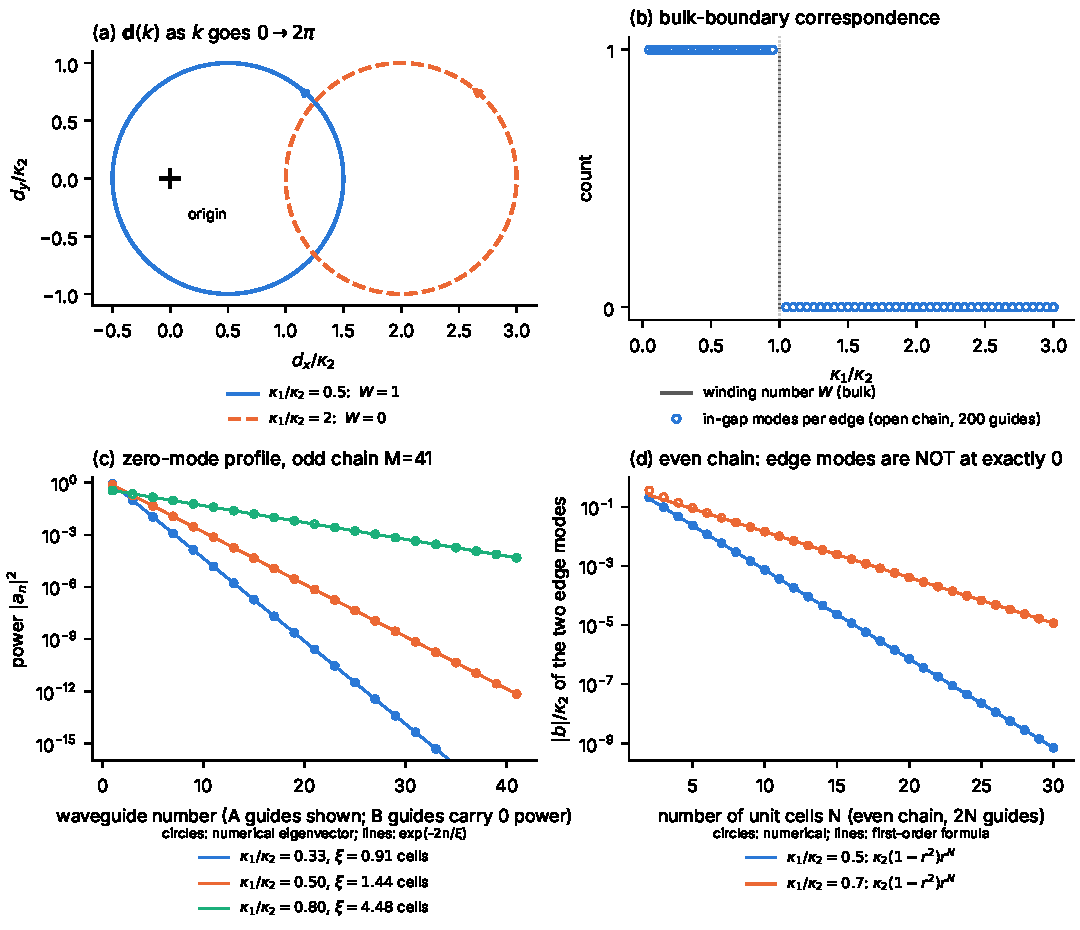
\includegraphics[width=0.92\linewidth]{../../figures/fig_topology.pdf}
\caption{Generated by \texttt{scripts/day2\_topology.py} from \texttt{data/day2\_topology.npz} (deterministic). (a) $\bm d(k)$ loops. (b) $W$ vs.\ in-gap modes per edge of a 200-guide chain. (c) Zero-mode power on the A guides of a 41-guide chain (circles: \texttt{eigh}; lines: $e^{-2n/\xi}$); the $r=1/3$ data stop at $10^{-16}$ = double-precision round-off. (d) Even-chain edge splitting vs.\ $N$.}
\label{fig:topo}
\end{figure}

%=====================================================================
\section{Physical scale: what the literature actually gives us}
%=====================================================================
From Blanco-Redondo \emph{et al.}, PRL \textbf{116}, 163901 (2016) \evd{Literature, read from the author-accepted manuscript}:
\begin{itemize}[itemsep=1pt]
\item Silicon-on-insulator waveguides, 450~nm $\times$ 220~nm, air cladding, $\lambda=1550$~nm; 203 waveguides; 500~$\mu$m long; deep-UV lithography (IMEC).
\item Narrow/wide gaps: 166/294~nm (``long-long'', topological interface) and 182/324~nm (``short-short'', trivial compound defect). Equidistant reference: 230~nm.
\item Reported coupling \emph{ratios} $\approx2.96$--$3.26$ and $0.31$--$0.34$. \textbf{Absolute $\kappa$ values are not given in the text.}
\item They use a \textbf{domain wall in the middle} of the array (an interface between two SSH chains with Zak phases 0 and $\pi$), not an array edge. The topological interface mode kept the same output over an 8~nm wavelength range; the trivial ``short-short'' defect supported two modes that beat, so its output changed with length and wavelength.
\end{itemize}
\textbf{Decisions.}
\textbf{D2:} baseline ratio $r=\ka/\kc=1/3$ (literature-based). \textbf{D3:} keep $\kappa$ dimensionless (lengths in units of $1/\kc$) until an absolute value is obtained from a cited source or our own mode-solver calculation (optional COMSOL extension). Do not invent a number.
\textbf{D4 (new, important for Day 3):} their \emph{interface} geometry plus their ``short-short'' trivial defect is a published, physically fair topological-vs-trivial pair. I recommend we adopt this geometry for the comparison: it launches light into the middle (no end-guide self-shift problem L1), and it has an experimental precedent.

%=====================================================================
\section{Back to the research question: what we have, and what we do not}
%=====================================================================
\begin{tabular}{@{}p{0.3\linewidth}p{0.62\linewidth}@{}}\toprule
Concept & Status after Day 2\\\midrule
Eigenvalue pinning & \textbf{Derived}: $b=0$ exactly for chiral perturbations (odd chain), for any strength --- even beyond gap closing.\\
Localisation & \textbf{Derived} for the clean chain; disordered behaviour is Hypothesis H2. Needs the gap.\\
Phase stability & \textbf{Not addressed.} $b=0$ is measured from $\beta_0$; the phase is $(\beta_0+b)L$, and $\beta_0$ is not protected.\\
Transport / output stability & \textbf{Not addressed.} A launched field also excites bulk modes (Day 5).\\
Circuit-level robustness & \textbf{Not addressed} (Days 8--10).\\\bottomrule
\end{tabular}

%=====================================================================
\section{Code, tests and two lessons}
%=====================================================================
\texttt{topq/topology.py}: \texttt{chiral\_operator}, \texttt{chiral\_violation}, \texttt{winding\_number}, \texttt{zero\_mode\_from\_couplings}, \texttt{edge\_mode}, \texttt{sublattice\_weights}, \texttt{ipr}, \texttt{fit\_localization\_length}, \texttt{xi\_analytic}, \texttt{even\_chain\_splitting}. \texttt{tests/test\_topology.py}: 31 new tests; whole suite \textbf{54 passed}.

\textbf{Lesson 1 --- an ``equivalent mutant''.} In the mutation test I changed $\Gamma$ to $-\Gamma$ and \emph{no} test failed. That is correct, not a weak test: $(-\Gamma)H(-\Gamma)=\Gamma H\Gamma$, so the overall sign of the chiral operator has no physical meaning. Three other injected bugs (wrong sign in the zero-mode recursion, $\xi$ off by 2, winding direction) were caught.

\textbf{Lesson 2 --- stale cache.} After restoring the file, tests briefly still failed: Python reused a cached compiled copy (\texttt{\_\_pycache\_\_}) because the restored file had the same size and timestamp second. Deleting \texttt{\_\_pycache\_\_} fixed it. If results ever look ``impossible'' after an edit, clear the cache first.

\section{Self-test (answer without notes)}
\begin{enumerate}[itemsep=1pt]
\item Why does a uniform shift $\delta\beta\mathbb1$ break chiral symmetry but a random change of every $\kappa_n$ does not?
\item Draw the $\bm d$-loop for $\ka=\kc$. Why is $W$ undefined there?
\item An odd chain with $\ka>\kc$: where is its zero mode, and on which sublattice?
\item Why does the counting argument need ``A couples only to B''? Give a perturbation that defeats it.
\item Even chain, $r=0.5$: how many unit cells do you need for the edge-mode splitting to be below $10^{-6}\kc$?
\item In one sentence: why does $b=0$ \emph{not} by itself mean the light's phase is protected?
\end{enumerate}
\end{document}
